\documentclass[letter,10.5pt]{article}
%%%%%%%%%%%%%%%%%%%%%%%%%%%%%%%%%%%%%%%%%%%%%%%%
% 2. Packages
%%%%%%%%%%%%%%%%%%%%%%%%%%%%%%%%%%%%%%%%%%%%%%%%

\usepackage[top = 2cm, bottom = 2cm, left = 2cm, right = 2cm]{geometry} 

% The following two packages - multirow and booktabs - are needed to create nice looking tables.
\usepackage{IEEEtrantools}
\usepackage{setspace}
\setlength{\parindent}{0in}

% Package to place figures where you want them.
\usepackage{float}

% The fancyhdr package let's us create nice headers.
\usepackage{fancyhdr}
\usepackage{array}
\usepackage{amsmath}
\usepackage{amssymb}
\usepackage[svgnames]{xcolor}
\usepackage{graphicx}
\usepackage{sectsty}
\usepackage[shortlabels]{enumitem}
\DeclareMathOperator*{\argmax}{arg\,max}
\DeclareMathOperator*{\argmin}{arg\,min}
\let\otheriint\iint
\let\iint\relax
%%%%%%%%%%%%%%%%%%%%%%%%%%%%%%%%%%%%%%%%%%%%%%%%
% 3. Header (and Footer)
%%%%%%%%%%%%%%%%%%%%%%%%%%%%%%%%%%%%%%%%%%%%%%%%

\pagestyle{fancy} 
\fancyhf{}
\lhead{\footnotesize ECON 330: Computational Homework 1}
\rhead{\footnotesize{\textit{Lumbanraja, Alvin U.}}} %<---- Fill in your lastnames.
\cfoot{\footnotesize \thepage} 

%%%%%%%%%%%%%%%%%%%%%%%%%%%%%%%%%%%%%%%%%%%%%%%%
% 4. Your document
%%%%%%%%%%%%%%%%%%%%%%%%%%%%%%%%%%%%%%%%%%%%%%%%
\begin{document}
\newcolumntype{P}[1]{>{\centering\arraybackslash}p{#1}}
\def\thesection{\Alph{section}}
\sectionfont{\fontsize{12}{15}\selectfont}


\thispagestyle{plain} % This command disables the header on the first page. 

\begin{tabular}{p{17cm}} % This is a simple tabular environment to align your text nicely 
{\large \bf Computational Homework 1} \\
ECON 330 (Theory of Income) \\ Fall 2019  \\ {\bf{Alvin U. Lumbanraja}}\\

\hline % \hline produces horizontal lines.
\\
\end{tabular} % Our tabular environment ends here.


\section{Theoretical Benchmark}

\textbf{Notes:}
\newline Throughout this exercise, I use the following assumption based on the information from the problem sets
\begin{table}[htbp]
\centering
\textbf{\caption{Parameters}}
\vspace{0.1cm}
\begin{tabular}{  p{3cm}  P{0.8cm} P{0.8cm} P{0.8cm} P{0.8cm} P{0.8cm}}
\hline\hline
\textbf{Parameter} 	& $\beta$ 	& $\alpha$	& $\delta $ 	& $z$ 	& $k_0$ \\  
\hline
\textbf{Values} 		&  0.98 	& 1/3			& 1			& 1		& 0.05$k_{ss}$ \\ 
\hline\hline
\end{tabular}
\end{table}


\begin{enumerate}
	
	%% 			A1
	
\item Given the functional form of the utility function, we know that:

\begin{itemize}
  \item  For every $k \in K$, we know that the feasible set is non-empty
  \item  Value function is monotone, concave, and differentiable
  \item  The policy function $g(k)$ is single-valued
\end{itemize}

By substituting $k_{t+1}$ as $k'$, substituting the value of $c_t$ as a function of $k_t$ and $k_{t+1}$, we can define the Bellman equation for this problem as 
\begin{IEEEeqnarray}{rCl} 
v(k) &=& \max_{k'\in\Gamma(k)} \{F(k,k')+\beta v(k')\} \IEEEnonumber 
\\ &=& \max_{k'\in\Gamma(k)} \{\ln[zk^\alpha+(1-\delta)k-k']+\beta v(k')\}  \quad\text{(Generalized form)}
\\ &=& \max_{k'\in\Gamma(k)} \{\ln[k^{\frac{1}{3}}-k']+\beta v(k')\} \quad\text{(with specified parameters)}
\end{IEEEeqnarray}

Let us also define the feasibility constraint $\Gamma$ in terms of $k$ and $k'$
\begin{IEEEeqnarray}{rCl} 
\Gamma(k) &\equiv& [0, (zk_t^\alpha + (1-\delta)k_t] \IEEEnonumber
\\ &\equiv& [0, k^{\frac{1}{3}}]
\end{IEEEeqnarray}

The capital is fully depreciated and owing to the fact that the function is in the log form, we can rule out corner solution, both on the lower bound and upper bound (both $c_t = k_t$, which means  $c'=k'^{\frac{1}{3}}=0$ and  $c_t = 0$ are not feasible)

	%% 			A2

\item Let $g(k)$ denotes the optimal choice for $k'$. The first order condition for this problem is as follows:
\begin{IEEEeqnarray}{rCl} 
0 &=&  \frac{\partial}{\partial k'} \ln[zk^{\alpha}+(1-\delta)k-g(k)] + \beta\frac{\partial}{\partial k} v(g(k)) \IEEEnonumber
\\ &=& \frac{\partial}{\partial k'} \ln[k^{\frac{1}{3}}-g(k)] + 0.98\frac{\partial}{\partial k} v(g(k)) \IEEEnonumber
\\ \IEEEnonumber
\\ &=& -\frac{1}{zk^{\alpha}+(1-\delta)k-g(k)} + \beta v'(g(k)) \leq 0 \quad\text{(Generalized form)}
\\ &=& -\frac{1}{(k^{\frac{1}{3}}-g(k))} + 0.98\frac{\partial}{\partial k} v(g(k)) \quad\text{(with specified parameters)}
\end{IEEEeqnarray}

The envelope condition is as follows:
\begin{IEEEeqnarray}{rCl} 
 \frac{\partial}{\partial k} v(k) &=& \frac{\partial}{\partial k} \ln[zk^\alpha+(1-\delta)k-g(k)]
 \\ \IEEEnonumber
 \\ v'(k) &=& \frac{\alpha z k^{\alpha-1} + (1-\delta)}{zk^{\alpha}+(1-\delta)k-g(k)}  \quad\text{(Generalized form)}
 \\ &=& -\frac{1}{3k^\frac{2}{3}(k^{\frac{1}{3}}-g(k))} \quad\text{(with specified parameters)}
\end{IEEEeqnarray}

The Euler equation is as follows:
\begin{IEEEeqnarray}{rCl} 
0 &=& \frac{\partial}{\partial k'} \ln[zk^{\alpha}+(1-\delta)k-g(k)] + \beta\frac{\partial}{\partial k} \ln[zg(k)^{\alpha}+(1-\delta)g(k)-g(g(k))] \IEEEnonumber
\\ &=& \frac{\partial}{\partial k'} \ln[k^{\frac{1}{3}}-g(k)] + 0.98\frac{\partial}{\partial k} \ln[g(k)^{\frac{1}{3}}-g(g(k))] \IEEEnonumber
\\ \IEEEnonumber
\\ &=& -\frac{1}{zk^{\alpha}+(1-\delta)k-g(k)} + \beta\Big[\frac{\alpha z g(k)^{\alpha-1} + (1-\delta)}{zg(k)^{\alpha}+(1-\delta)g(k)-g(g(k))}   \Big]
\\ &=& -\frac{1}{(k^{\frac{1}{3}}-g(k))} + \frac{0.98}{3g(k)^\frac{2}{3}(k^{\frac{1}{3}}-g(k))}
\end{IEEEeqnarray}

The optimal policy function can be recursively written as:
\begin{IEEEeqnarray}{rCl} 
\frac{1}{k^{\frac{1}{3}}-g(k)} &=&  \frac{0.98}{3g(k)^\frac{2}{3}(g(k)^{\frac{1}{3}}-g(g(k)))} \IEEEnonumber
\\ g(k)^{\frac{1}{3}}-g(g(k)) &=& \frac{0.98(k^{\frac{1}{3}}-g(k))}{3g(k)^\frac{2}{3}} \IEEEnonumber
\\ g(g(k)) &=& g(k)^{\frac{1}{3}} - \frac{0.98(k^{\frac{1}{3}}-g(k))}{3g(k)^\frac{2}{3}} \IEEEnonumber
\\ g(k) &=& k^{\frac{1}{3}} - \frac{0.98(k_{t-1}^{\frac{1}{3}}-k)}{3k^\frac{2}{3}} \IEEEnonumber
\\ &=& k^{\frac{1}{3}} - \frac{0.98(k_{t-1}^{\frac{1}{3}}-k)}{3k^\frac{2}{3}}
\end{IEEEeqnarray}

It may be difficult to show algebraically how $g(k)$ reacts to change in $k_0$. However, by concavity of the return function $F$, we know that approximate policy functions $\{g(k)\}$ converges pointwise. Therefore, the sequence of policy function $\{g(k)\}$ will increase if $k_0$ increase when $k_0<k_ss$, and vice-versa.

	%% 			A3
	
\item Using the Euler equation, let us define steady state level capital where $k=g(k)=k_{ss}$
\begin{IEEEeqnarray}{rCl} 
k_{ss} &=& \left[ \frac{1-\beta(1-\delta)}{\beta \alpha z} \right]^{\frac{1}{\alpha-1}}
\\ \IEEEnonumber
\\ k_{ss} &=& \Big( \frac{3}{0.98} \Big)^{\frac{3}{2}} \approx 0.1867
\end{IEEEeqnarray}

	%% 			A4
\item	Let us assume that the value function $v(k)$ equals to certain value of the functional form $a \log(k) + b$. We then know that:
\begin{IEEEeqnarray}{rCl} 
v'(k) &=& \frac{a}{k} \IEEEnonumber
\end{IEEEeqnarray}

Notice that this is similar to the envelope condition. Recall the general form of for this problem
\begin{IEEEeqnarray}{rCl} 
v'(k) &=& \frac{\alpha z k^{\alpha-1} + (1-\delta)}{zk^{\alpha}+(1-\delta)k-g(k)} \IEEEnonumber
\end{IEEEeqnarray}

Setting the value equal, we obtain
\begin{IEEEeqnarray}{rCl} 
\frac{a}{k} &=& \frac{\alpha z k^{\alpha-1} + (1-\delta)}{zk^{\alpha}+(1-\delta)k-g(k)} 
\end{IEEEeqnarray}

By exploiting the fact that $\delta=1$, we can further reduce the equation () to 
\begin{IEEEeqnarray}{rCl} 
\frac{a}{k} &=& \frac{\alpha z k^{\alpha-1}}{zk^{\alpha}-g(k)}  = \frac{\alpha z}{zk-\frac{g(k)}{k^{\alpha-1}}} 
\end{IEEEeqnarray}

However, for the equation above to be consistent, we then need the equation above to be in the form of 
\begin{IEEEeqnarray}{rCl} 
\frac{a}{k} &=& \frac{\alpha z}{zk-\frac{g(k)}{k^{\alpha-1}}}  = \frac{\alpha z}{(z-\gamma)k} 
\end{IEEEeqnarray}

So that
\begin{IEEEeqnarray}{rCl} 
\gamma k &=& \frac{g(k)}{k^{\alpha-1}}
\\ g(k) &=& \gamma k^\alpha
\end{IEEEeqnarray}

By plugging the value to our FOC, we obtain
\begin{IEEEeqnarray}{rCl} 
\gamma &=& \frac{\beta \alpha z^2}{z-\gamma + \beta\alpha z} \IEEEnonumber
\\ (\gamma-z)(\gamma-\alpha\beta z) &=& 0
\end{IEEEeqnarray}

The only logical value for $\gamma$ is therefore $\gamma=\alpha\beta z$. Therefore, we may compute the following
\begin{IEEEeqnarray}{rCl} 
a &=& \frac{\alpha}{1-\alpha\beta}
\\g(k) &=& \alpha\beta zk^\alpha
\\ v(k) &=& \frac{\alpha}{1-\alpha\beta}\ln(k)+b
\end{IEEEeqnarray}

We are thus interested in knowing the value of $b$. By setting the $b$ equal to the value function
\begin{IEEEeqnarray}{rCl} 
a\ln(k)+b &=& \ln[zk^\alpha+(1-\delta)k-k']+\beta(\ln k' + b) \IEEEnonumber
\\ b &=& \frac{\ln[zk^\alpha+(1-\delta)k-k']+\beta(a)-a\ln(k)}{1-\beta} \IEEEnonumber
\\ &=& \frac{\ln[zk^\alpha+(1-\delta)k-k']+\beta(a)-a\ln(k)}{1-\beta} \IEEEnonumber
\\ &=& \frac{\ln(z(1-\alpha\beta))+\frac{\alpha\beta}{1-\alpha\beta}\ln(\alpha\beta)}{1-\beta}
\end{IEEEeqnarray}

We thus can conclude that $a$ and $b$ can indeed be constant, and the value function is in the form of 
\begin{IEEEeqnarray}{rCl} 
v(k) &=& \frac{\alpha}{1-\alpha\beta}\ln(k)+\frac{\ln(z(1-\alpha\beta))+\frac{\alpha\beta}{1-\alpha\beta}\ln(\alpha\beta)}{1-\beta}
\end{IEEEeqnarray}

\newpage
We can plot analytically the value of $v(k)$ and $g(k)$ as follows:
\begin{figure}[hbtp]
\centering
\caption{Analytical Simulation}
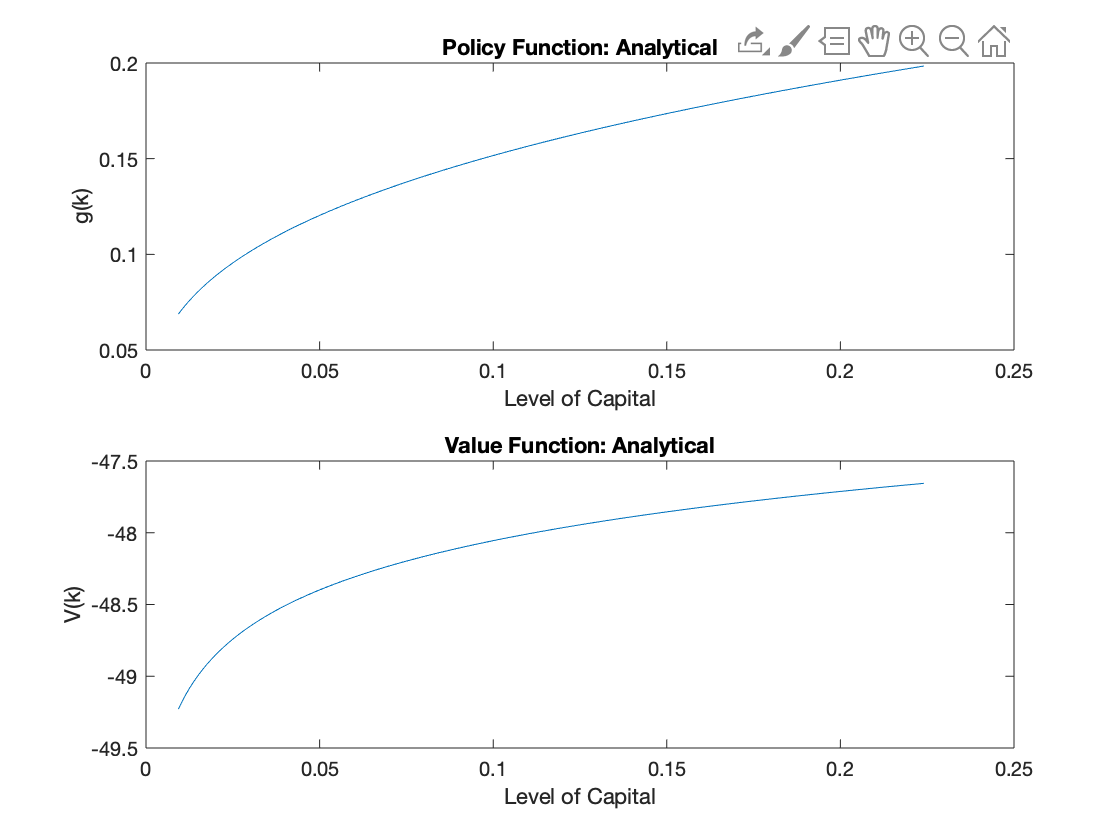
\includegraphics[scale=0.27]{part_a.png}
\end{figure}


\end{enumerate}


\section{Brute Force Value Function Iteration}
The amount of time it takes to run this algorithm (measured from starting the grid of capital until the end) is 5.0543s. The result (shown below) is similar to (A)
\begin{figure}[hbtp]
\centering
\caption{Brute Force Value Function Simulation}
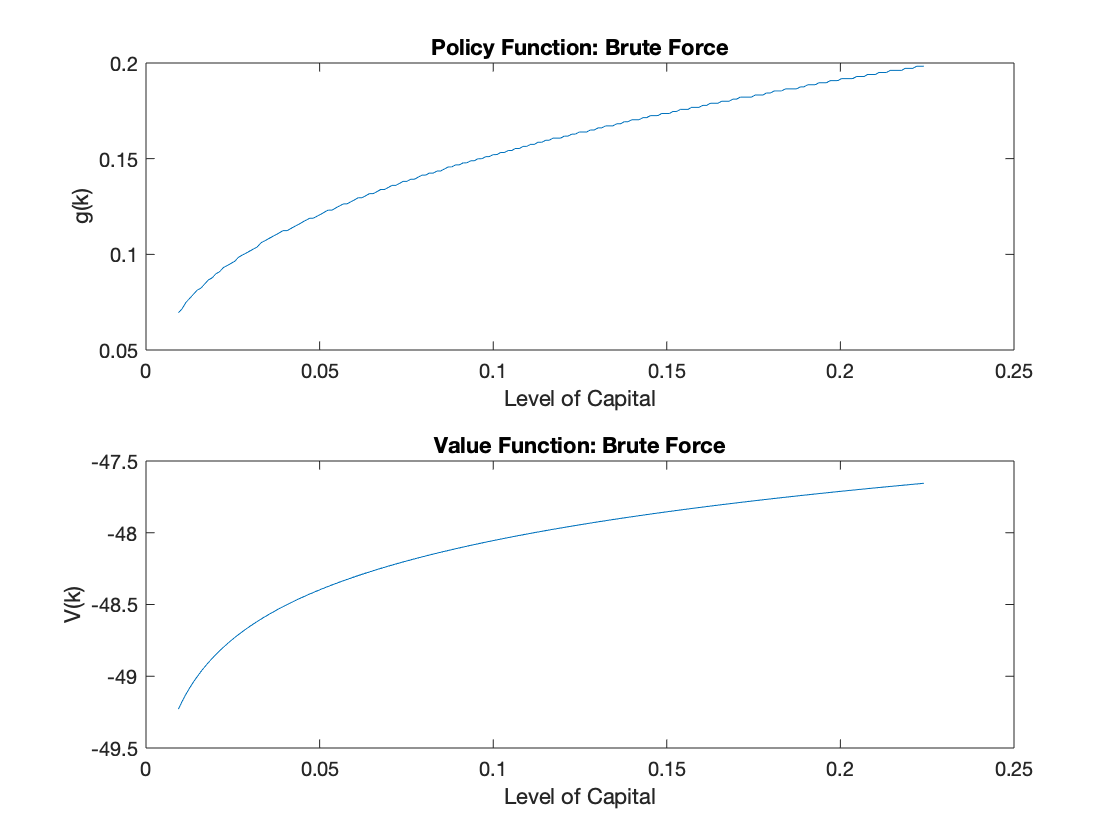
\includegraphics[scale=0.27]{part_b.png}
\end{figure}


\section{Improved Guess in $V_0$}

The amount of time it takes to run this algorithm (measured from starting the grid of capital until the end) is 0.1018s. The result (shown below) is similar to (A). The interpretation for the $V_0$ guess is that the value function should be proportional to the value of the return function. 
\begin{figure}[hbtp]
\centering
\caption{Improved Guess in $V_0$ Simulation}
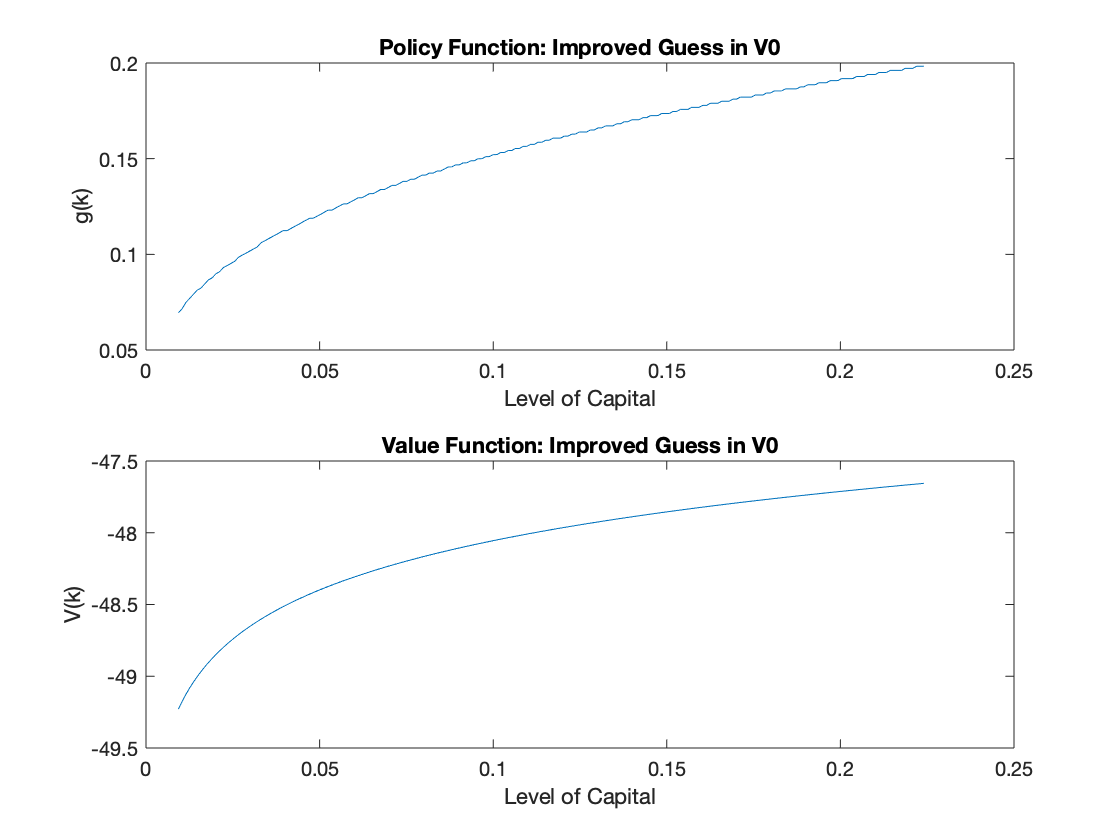
\includegraphics[scale=0.27]{part_c.png}
\end{figure}


\section{Improved Decision Process}
The amount of time it takes to run this algorithm (measured from starting the grid of capital until the end) is 2.4361s. The result (shown below) is similar to (A). Compared to the brute force, this algorithm is significantly faster (almost 52\% faster), but still slower than educated guess of the value function.
\begin{figure}[hbtp]
\centering
\caption{Improved Decision Process}
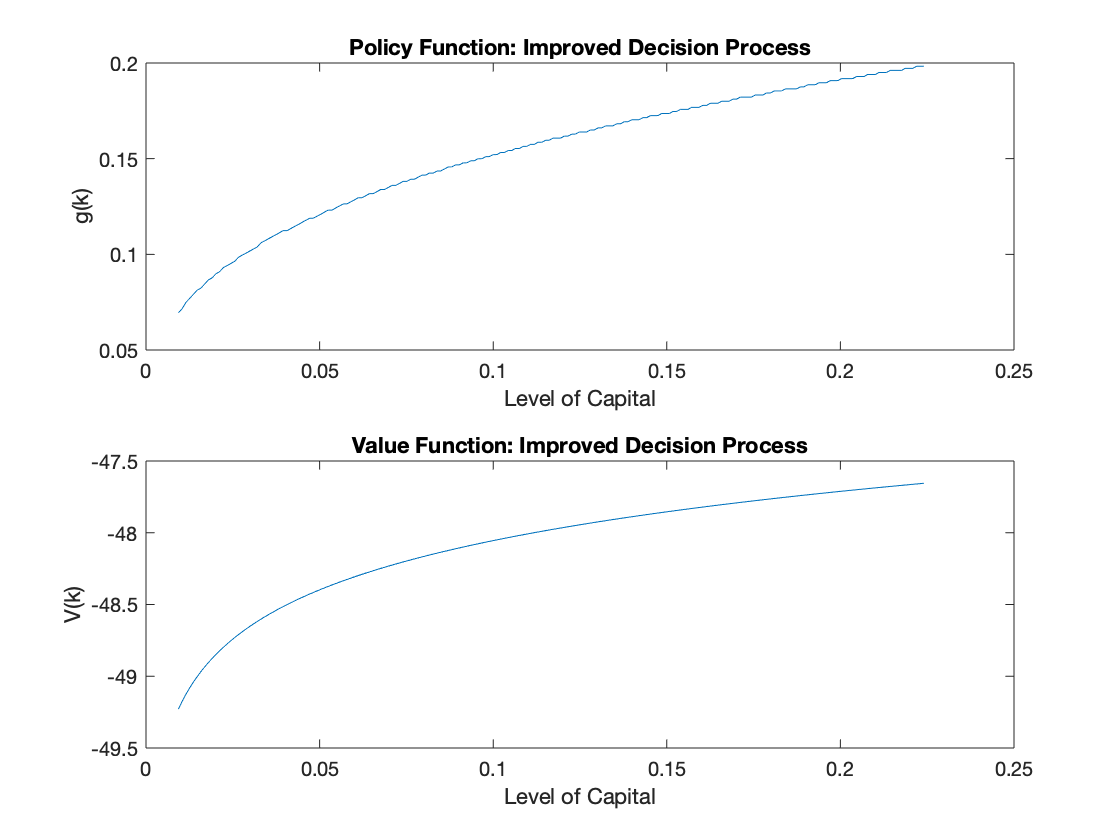
\includegraphics[scale=0.27]{part_d.png}
\end{figure}


\section{Storing the Return Function}
The amount of time it takes to run this algorithm (measured from starting the grid of capital until the end) is 0.1967s. The result (shown below) is similar to (A). Compared to the brute force, this algorithm is significantly faster (more than 96\% faster), but still slower than educated guess of the value function.
\begin{figure}[hbtp]
\centering
\caption{Storing the Return Function}
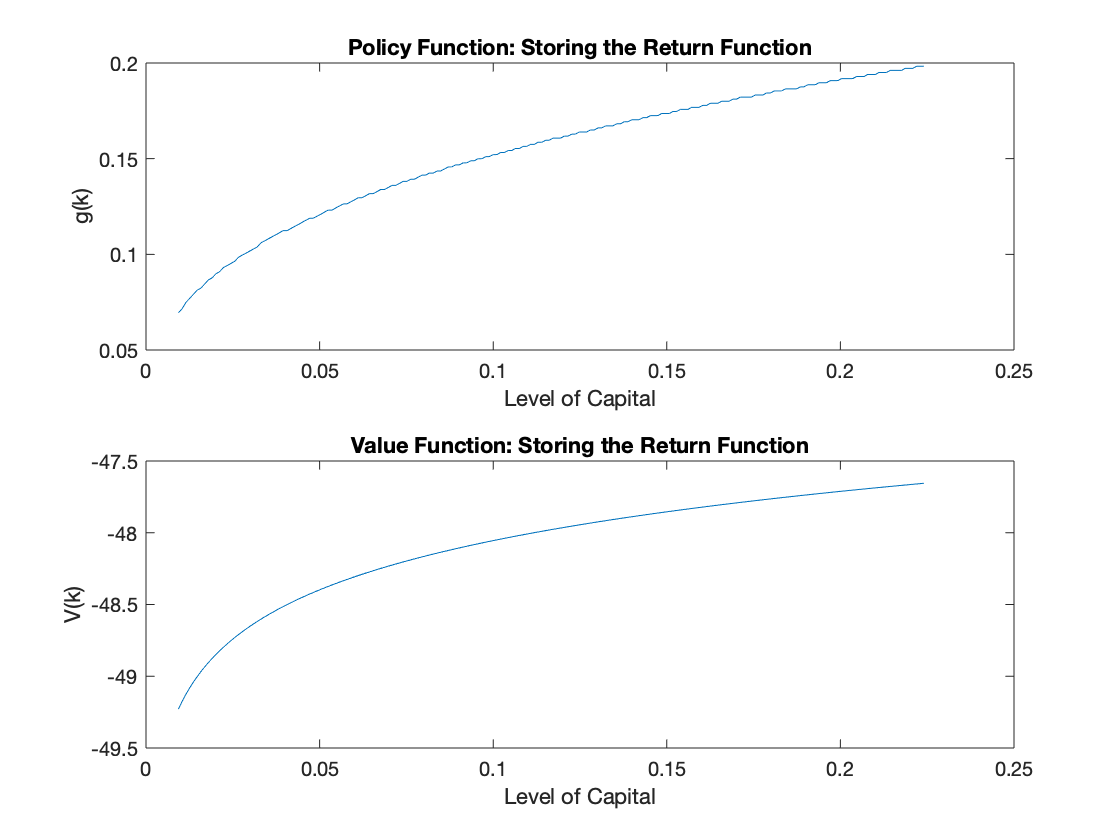
\includegraphics[scale=0.27]{part_e.png}
\end{figure}

\section{Howard's Improvement Algorithm}
The amount of time it takes to run this algorithm (measured from starting the grid of capital until the end) is 0.2791s. The result (shown below) is similar to (A). Compared to the brute force, this algorithm is significantly faster (more than 94\% faster), but still slower than educated guess of the value function.
\begin{figure}[hbtp]
\centering
\caption{Howard's Improvement Algorithm}
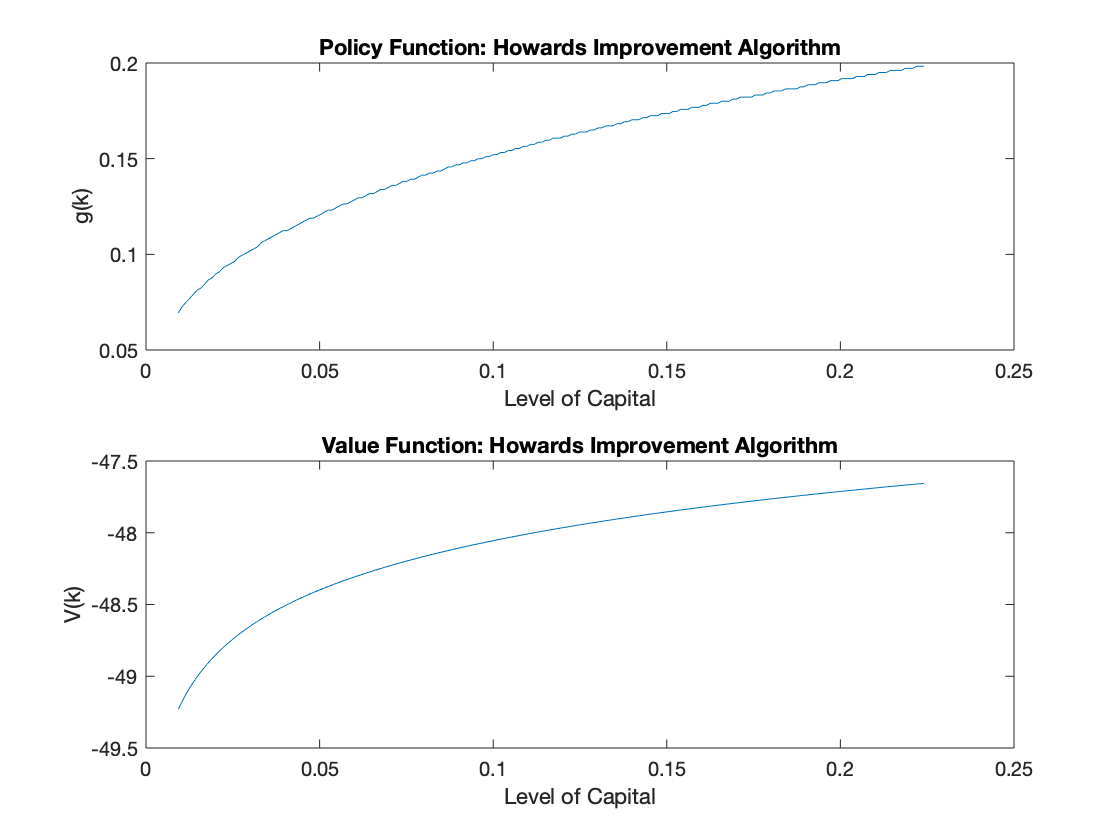
\includegraphics[scale=0.27]{part_f.png}
\end{figure}

\section{Combining Methods and Concluding Notes}
The amount of time it takes to run this algorithm (measured from starting the grid of capital until the end) is 0.0714s. The result (shown below) is similar to (A). Compared to the brute force, this algorithm is significantly faster (more than 98\% faster). This is the only algorithm that is faster than educated guess of the value function.
\begin{figure}[hbtp]
\centering
\caption{Howard's Improvement Algorithm}
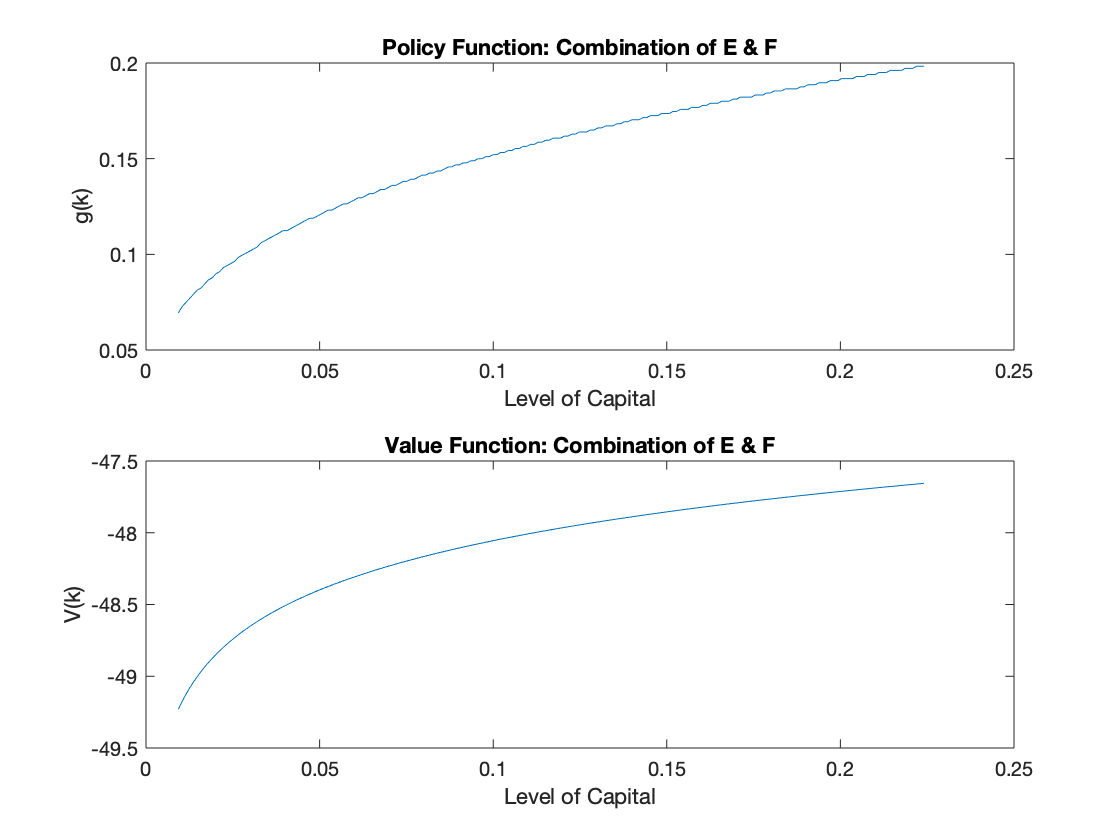
\includegraphics[scale=0.27]{part_g.png}
\end{figure}


\begin{table}[htbp]
\centering
\textbf{\caption{Algorithm Performance}}
\vspace{0.3cm}
\begin{tabular}{  p{6cm}  P{2cm}  P{2cm} } 
\hline\hline
\textbf{Parameter}& \textbf{Iteration} & \textbf{Time} \\ 
\hline
B. Brute Force  				& 570 & 5.0543 \\ 

C. Improved Guess in $V_0$			& 7 & 0.1018 \\ 

D. Improved Decision Process			& 570 & 2.4361 \\ 

E. Storing the Return Function			& 570 & 0.1967 \\ 

F. Howard's Improvement Algorithm		& 23 & 0.2791  \\ 

G. Combination of E \& F				& 23 & 0.0714  \\ 
\hline\hline
\end{tabular}
\vspace{1ex}

{\raggedright \footnotesize{Computation done on 2017 MacBook Pro 13", 3.1 GHz Intel Core i5}}
\end{table}

The algorithm performance highly depends on (1) the initial guess on the optimal value of capital and (2) the efficiency of algorithm. Having more efficient algorithm can significantly reduce the needed iteration; by not performing unnecessary looping and/or performing maximization every time we perform iteration, we can cut down significantly on the need for computational power. However, the most significant time saving is provided by having an educated guess prior to performing algorithm. Even with the most inefficient algorithm, having a good guess on the value function will cut down the necessary iteration significantly.



\end{document}